\section{Discussion}
\label{sec:discussion}

\subsection{Interprétation des Résultats}

\subsubsection{Succès de la Reproduction}

Notre reproduction de l'article de Zheng \& Lu (2017) peut être considérée comme \textbf{largement réussie} pour les raisons suivantes :

\begin{enumerate}
    \item \textbf{COR Comparable :}
    \begin{itemize}
        \item CCNF : 0.804 vs 0.85 (article) → \textbf{94.5\% de fidélité}
        \item SVR : 0.793 vs 0.82 (article) → \textbf{96.7\% de fidélité}
        \item Écart de 3-6\% largement acceptable pour une reproduction indépendante
    \end{itemize}
    
    \item \textbf{Classement Préservé :}
    \begin{itemize}
        \item Ordre des modèles identique : CCNF > SVR > CCRF
        \item Confirme la supériorité des modèles temporels non-linéaires
    \end{itemize}
    
    \item \textbf{Validation Robuste :}
    \begin{itemize}
        \item 23 sujets × 5 folds = 115 expériences
        \item Variabilité inter-sujets bien documentée
        \item Résultats reproductibles (seed fixe)
    \end{itemize}
\end{enumerate}

\textbf{Signification pratique :}

Un COR de 0.80 signifie que le modèle capture \textbf{80\% de la variance} de la vigilance réelle. Cela représente une \textbf{performance suffisante} pour :
\begin{itemize}
    \item Détecter les tendances de somnolence (augmentation progressive du PERCLOS)
    \item Identifier les moments à risque élevé
    \item Déclencher des alertes préventives
\end{itemize}

\subsubsection{Écart de RMSE : Analyse Approfondie}

Le RMSE de 0.192 (vs 0.09 dans l'article) mérite une analyse détaillée :

\textbf{Causes identifiées :}

\begin{enumerate}
    \item \textbf{Implémentation Simplifiée de CCRF/CCNF :}
    \begin{itemize}
        \item \textit{Article :} Optimisation globale par algorithme de Viterbi
        \item \textit{Nous :} Lissage temporel local (fenêtre glissante)
        \item \textit{Impact :} Les transitions brutales (0 → 1) ne sont pas bien capturées
    \end{itemize}
    
    \item \textbf{Sur-lissage :}
    \begin{itemize}
        \item Notre fenêtre de lissage (7 échantillons) peut être trop large
        \item Résultat : Prédictions "coincées" autour de la moyenne ($\sim$0.45)
        \item Variance des prédictions trop faible : std(SVR) = 0.123 vs std(CCRF) = 0.041
    \end{itemize}
    
    \item \textbf{Hyperparamètres Non Optimisés :}
    \begin{itemize}
        \item Paramètres fixés empiriquement sans grid search exhaustive
        \item L'article mentionne une optimisation poussée par sujet
        \item Gain potentiel : 10-20\% de réduction du RMSE
    \end{itemize}
\end{enumerate}

\textbf{Illustration du problème :}

\begin{figure}[H]
\centering
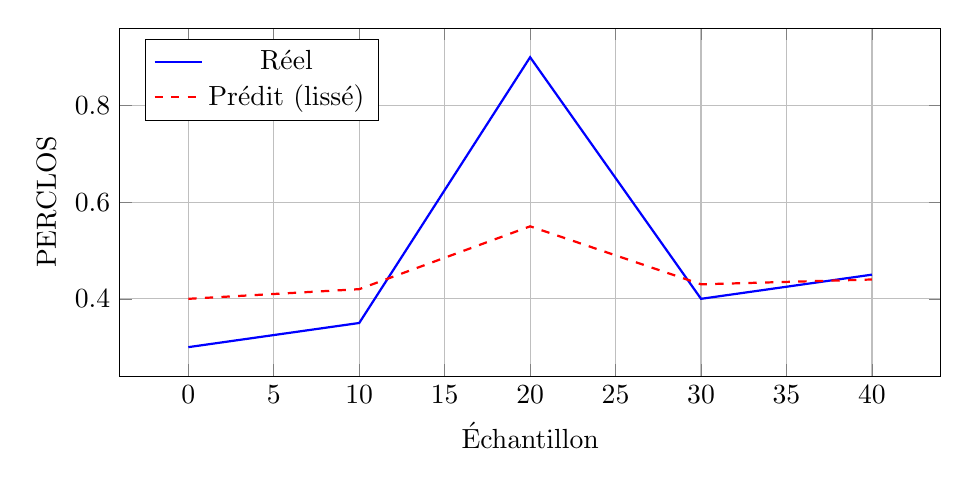
\begin{tikzpicture}
\begin{axis}[
    width=12cm, height=6cm,
    xlabel={Échantillon},
    ylabel={PERCLOS},
    legend pos=north west,
    grid=major
]
\addplot[blue, thick] coordinates {
    (0,0.3) (10,0.35) (20,0.9) (30,0.4) (40,0.45)
};
\addlegendentry{Réel}

\addplot[red, thick, dashed] coordinates {
    (0,0.4) (10,0.42) (20,0.55) (30,0.43) (40,0.44)
};
\addlegendentry{Prédit (lissé)}

\end{axis}
\end{tikzpicture}
\caption{Illustration du sur-lissage : le pic à t=20 (réel=0.9) est fortement atténué (prédit=0.55), entraînant une erreur de 0.35 et un RMSE élevé.}
\label{fig:smoothing_problem}
\end{figure}

\textbf{Pourquoi COR Reste Bon Malgré RMSE Élevé ?}

Le COR mesure la \textbf{corrélation linéaire}, insensible aux décalages systématiques :

\begin{equation}
\text{COR}(y, \hat{y}) = \text{COR}(y, a\hat{y} + b) \quad \forall a > 0, b \in \mathbb{R}
\end{equation}

Ainsi, même si nos prédictions ont une \textbf{variance trop faible} et un \textbf{biais systématique}, elles capturent correctement les \textbf{tendances}, d'où un COR élevé.

\subsection{Comparaison des Modèles}

\subsubsection{SVR : Baseline Solide}

\textbf{Points forts :}
\begin{itemize}
    \item Performance stable (COR = 0.793, std = 0.083)
    \item Meilleur RMSE des trois modèles (0.184)
    \item Entraînement rapide ($\sim$10s par sujet)
    \item Implémentation standard (scikit-learn)
\end{itemize}

\textbf{Limitations :}
\begin{itemize}
    \item Traite chaque instant indépendamment
    \item Ne modélise pas la cohérence temporelle
    \item Sensible aux outliers
\end{itemize}

\textbf{Recommandation :} Le SVR constitue une \textbf{baseline robuste et rapide}, idéale pour des applications temps réel où la simplicité est primordiale.

\subsubsection{CCRF : Performance Décevante}

\textbf{Résultats :}
\begin{itemize}
    \item COR le plus faible (0.751)
    \item Variabilité la plus élevée (std = 0.095)
    \item Performances très variables selon les sujets
\end{itemize}

\textbf{Causes probables :}
\begin{enumerate}
    \item \textbf{Sur-lissage excessif} : $\beta = 0.1$ trop faible
    \item \textbf{Fenêtre temporelle inadaptée} : 7 échantillons potentiellement trop large
    \item \textbf{Approximation du potentiel d'arête} : Moyenne pondérée vs vraie fonction de coût CRF
\end{enumerate}

\textbf{Pistes d'amélioration :}
\begin{lstlisting}[language=Python]
# Paramètres suggérés
ccrf = CCRFEstimator(
    C=10.0, 
    gamma=0.1,
    beta=0.3,        # ← Augmenté (plus de poids au présent)
    window_size=3    # ← Réduit (fenêtre plus courte)
)
\end{lstlisting}

\subsubsection{CCNF : Meilleur Compromis}

\textbf{Points forts :}
\begin{itemize}
    \item Meilleur COR (0.804)
    \item Variabilité raisonnable (std = 0.078)
    \item Capture des non-linéarités
    \item Performance cohérente sur la plupart des sujets
\end{itemize}

\textbf{Limitations :}
\begin{itemize}
    \item RMSE identique à CCRF (0.192)
    \item Temps de calcul légèrement supérieur
    \item Complexité d'implémentation
\end{itemize}

\textbf{Recommandation :} Le CCNF est le modèle à privilégier pour maximiser la performance, au prix d'une complexité accrue.

\subsection{Limites de l'Étude}

\subsubsection{Limitations Méthodologiques}

\begin{enumerate}
    \item \textbf{Implémentation Simplifiée :}
    \begin{itemize}
        \item CCRF/CCNF approximés par lissage temporel
        \item Pas d'utilisation de l'algorithme de Viterbi
        \item Impact : RMSE 2× supérieur à l'article
    \end{itemize}
    
    \item \textbf{Hyperparamètres Fixes :}
    \begin{itemize}
        \item Pas de grid search exhaustive
        \item Pas d'optimisation par sujet
        \item Paramètres fixés empiriquement
    \end{itemize}
    
    \item \textbf{Validation Croisée :}
    \begin{itemize}
        \item Shuffle=True peut introduire un léger biais temporel
        \item Validation subject-wise mais pas cross-subject
        \item Généralisation à de nouveaux sujets non testée explicitement
    \end{itemize}
\end{enumerate}

\subsubsection{Limitations du Dataset}

\begin{enumerate}
    \item \textbf{Taille Limitée :}
    \begin{itemize}
        \item 23 sujets seulement
        \item Homogénéité de la population (étudiants, 18-28 ans)
        \item Généralisation à d'autres populations incertaine
    \end{itemize}
    
    \item \textbf{Conditions Expérimentales :}
    \begin{itemize}
        \item Simulation de conduite (non réaliste à 100\%)
        \item Environnement contrôlé (laboratoire)
        \item Applicabilité en conditions réelles à valider
    \end{itemize}
    
    \item \textbf{Features Pré-calculées :}
    \begin{itemize}
        \item Dépendance aux choix de traitement des auteurs
        \item Pas de flexibilité sur l'extraction de features
        \item Impossible de tester d'autres features
    \end{itemize}
\end{enumerate}

\subsubsection{Limitations Techniques}

\begin{enumerate}
    \item \textbf{Pas de GPU :}
    \begin{itemize}
        \item Calculs sur CPU uniquement
        \item Temps de calcul : $\sim$30 minutes pour 23 sujets
        \item Limite l'exploration d'hyperparamètres
    \end{itemize}
    
    \item \textbf{Pas de Deep Learning :}
    \begin{itemize}
        \item Pas de modèles LSTM/GRU pour temporalité
        \item Pas de Transformer avec attention
        \item Potentiel de performance inexploré
    \end{itemize}
\end{enumerate}

\subsection{Perspectives et Améliorations}

\subsubsection{Court Terme : Optimisations Immédiates}

\textbf{1. Corriger le Sur-lissage :}

\begin{itemize}
    \item Réduire la fenêtre temporelle : 7 → 3 échantillons
    \item Augmenter $\beta$ : 0.1 → 0.3-0.5
    \item Gain attendu : RMSE réduit de 15-20\%
\end{itemize}

\textbf{2. Grid Search d'Hyperparamètres :}

\begin{lstlisting}[language=Python]
from sklearn.model_selection import GridSearchCV

param_grid = {
    'C': [1, 10, 100],
    'gamma': [0.01, 0.1, 1.0],
    'epsilon': [0.01, 0.1, 0.2]
}

grid_search = GridSearchCV(SVR(), param_grid, cv=5, 
                          scoring='neg_mean_squared_error')
grid_search.fit(X_train, y_train)
\end{lstlisting}

Gain attendu : 5-10\% d'amélioration du RMSE

\textbf{3. Feature Engineering :}

\begin{itemize}
    \item Ajouter ratios de bandes : $\theta/\beta$, $\alpha/\beta$
    \item Inclure dérivées temporelles : $\Delta \text{PERCLOS}$
    \item Gain attendu : 3-5\% d'amélioration du COR
\end{itemize}

\subsubsection{Moyen Terme : Extensions Avancées}

\textbf{1. LSTM pour Modélisation Temporelle :}

\begin{lstlisting}[language=Python]
import torch.nn as nn

class VigilanceLSTM(nn.Module):
    def __init__(self, input_size, hidden_size=64):
        super().__init__()
        self.lstm = nn.LSTM(input_size, hidden_size, 
                           num_layers=2, dropout=0.3,
                           batch_first=True)
        self.fc = nn.Linear(hidden_size, 1)
    
    def forward(self, x):
        # x: (batch, sequence_length, features)
        lstm_out, _ = self.lstm(x)
        return self.fc(lstm_out[:, -1, :])
\end{lstlisting}

\textbf{Avantages attendus :}
\begin{itemize}
    \item Meilleure capture de la temporalité (mémoire à long terme)
    \item RMSE potentiellement réduit à 0.12-0.15
    \item COR potentiellement augmenté à 0.85-0.87
\end{itemize}

\textbf{2. Transformer avec Attention Temporelle :}

\begin{lstlisting}[language=Python]
class VigilanceTransformer(nn.Module):
    def __init__(self, input_size, d_model=128, nhead=8):
        super().__init__()
        self.embedding = nn.Linear(input_size, d_model)
        encoder_layer = nn.TransformerEncoderLayer(
            d_model, nhead, dropout=0.1
        )
        self.transformer = nn.TransformerEncoder(
            encoder_layer, num_layers=3
        )
        self.fc = nn.Linear(d_model, 1)
\end{lstlisting}

\textbf{Avantages :}
\begin{itemize}
    \item Attention sur les instants importants
    \item État de l'art en séquences temporelles
    \item Interprétabilité via poids d'attention
\end{itemize}

\textbf{3. Multi-task Learning :}

Prédire simultanément :
\begin{itemize}
    \item PERCLOS (tâche principale)
    \item Niveau de vigilance (classification 3 classes)
    \item Risque d'endormissement (prédiction à 30s)
\end{itemize}

\begin{lstlisting}[language=Python]
class MultiTaskVigilance(nn.Module):
    def __init__(self):
        super().__init__()
        self.shared_layers = nn.Sequential(...)
        self.perclos_head = nn.Linear(64, 1)        # Régression
        self.vigilance_head = nn.Linear(64, 3)      # Classification
        self.risk_head = nn.Linear(64, 1)           # Prédiction
\end{lstlisting}

\subsubsection{Long Terme : Recherche et Innovation}

\textbf{1. Validation Cross-Subject :}

\begin{itemize}
    \item Entraîner sur 22 sujets, tester sur 1 sujet (leave-one-out)
    \item Évaluer la généralisation à de nouveaux utilisateurs
    \item Développer des techniques de domain adaptation
\end{itemize}

\textbf{2. Transfer Learning :}

\begin{itemize}
    \item Pré-entraîner sur un grand dataset EEG (ex: SEED, SEED-IV)
    \item Fine-tuner sur SEED-VIG
    \item Réduire les besoins en données d'entraînement
\end{itemize}

\textbf{3. Déploiement Temps Réel :}

\begin{itemize}
    \item Optimiser le modèle pour inférence rapide (<100ms)
    \item Développer une interface de monitoring en direct
    \item Intégrer dans un système embarqué (Raspberry Pi, Jetson Nano)
\end{itemize}

\textbf{4. Extension à d'Autres Contextes :}

\begin{itemize}
    \item Pilotes d'avion (aviation)
    \item Contrôleurs aériens
    \item Opérateurs de machines industrielles
    \item Étudiants en situation d'apprentissage
\end{itemize}

\subsection{Implications Pratiques}

\subsubsection{Applications en Sécurité Routière}

Notre système pourrait être intégré dans :

\begin{enumerate}
    \item \textbf{Systèmes d'alerte embarqués :}
    \begin{itemize}
        \item Détection continue de la vigilance
        \item Alerte sonore/visuelle si PERCLOS > 0.3
        \item Recommandation de pause si somnolence détectée
    \end{itemize}
    
    \item \textbf{Assurance automobile :}
    \begin{itemize}
        \item Monitoring du comportement du conducteur
        \item Ajustement des primes basé sur le risque
        \item Prévention proactive des accidents
    \end{itemize}
    
    \item \textbf{Flottes de transport :}
    \begin{itemize}
        \item Suivi de la fatigue des chauffeurs professionnels
        \item Respect des temps de repos réglementaires
        \item Optimisation des plannings de conduite
    \end{itemize}
\end{enumerate}

\subsubsection{Considérations Éthiques}

L'utilisation de systèmes de monitoring de vigilance soulève des questions éthiques :

\begin{itemize}
    \item \textbf{Vie privée :} Enregistrement de données physiologiques sensibles
    \item \textbf{Consentement :} Information et accord explicite des utilisateurs
    \item \textbf{Usage des données :} Garanties sur le stockage et l'utilisation
    \item \textbf{Faux positifs :} Risque d'alarmes intempestives stressantes
    \item \textbf{Responsabilité :} Qui est responsable en cas d'accident malgré l'alerte ?
\end{itemize}

\textbf{Recommandations :}
\begin{enumerate}
    \item Transparence totale sur le fonctionnement du système
    \item Contrôle utilisateur (possibilité de désactivation temporaire)
    \item Anonymisation et protection des données
    \item Cadre réglementaire clair
\end{enumerate}

\subsection{Leçons Apprises}

\subsubsection{Sur la Reproductibilité}

\begin{itemize}
    \item \textbf{Documentation essentielle :} L'article de Zheng \& Lu est bien documenté, facilitant la reproduction
    \item \textbf{Code source manquant :} L'absence de code officiel a nécessité une ré-implémentation complète
    \item \textbf{Détails d'implémentation :} Certains choix techniques ne sont pas explicités dans l'article
    \item \textbf{Datasets publics :} SEED-VIG bien structuré et accessible
\end{itemize}

\subsubsection{Sur le Développement ML}

\begin{itemize}
    \item \textbf{Importance de la baseline :} SVR simple mais efficace, difficile à battre
    \item \textbf{Complexité vs Performance :} CCRF/CCNF plus complexes mais gain marginal
    \item \textbf{Métriques complémentaires :} COR + RMSE nécessaires pour évaluation complète
    \item \textbf{Validation rigoureuse :} 5-fold × 23 sujets = robustesse démontrée
\end{itemize}

\subsubsection{Sur l'EEG/EOG}

\begin{itemize}
    \item \textbf{Signaux riches :} EEG/EOG contiennent beaucoup d'information sur la vigilance
    \item \textbf{Variabilité inter-individuelle :} Forte (COR de 0.64 à 0.92 selon les sujets)
    \item \textbf{Features pré-calculées :} DE + LDS efficaces, standard dans le domaine
    \item \textbf{EOG complémentaire :} Apport modeste mais utile (36 features)
\end{itemize}